% Copyright (c) 2014,2016 Casper Ti. Vector
% Public domain.

\chapter{引言}

\section{分布式图处理系统}
互联网的飞速发展产生了海量的数据,特别是最近几年智能移动设备的快速普及,更使得数据呈爆炸式增长。在大数据时代,海量数据的处理需求已远超单台机器所能提供的性能,为此人们在廉价的商用机集群上构筑了各式各样的分布式系统,以获得可靠、可扩展的海量数据处理能力。在各种数据表示方式中,图(Graph)由于其丰富的表达能力而得到了广泛应用。图中的顶点可以表示实体,图中的边表示实体间的关系。社交网络、语义网络、生物信息网络是典型的图应用场景。
图数据分析与处理是大数据背景下的一大研究分支\supercite{big_data},大数据背景下的图处理系统可以分为图计算框架和图数据库两大类。

图计算框架旨在高效地进行全图量级的并行计算,如计算PageRank\supercite{pagerank}、社区发现\supercite{community_detection}(Community Detection)、子图匹配\supercite{subgraph_listing}等,提供的是对OLAP(Online Analytical Processing)的支持。这类系统中,Pregel\supercite{pregel}、GraphLab\supercite{graphlab}、PowerGraph\supercite{powergraph}支持BSP\supercite{BSP}(Bulk Synchronous Parallel)模型的计算,对图数据进行特定的分割,使得集群中的机器可以在内存中计算分区的数据,再通过交互完成全量数据的计算。上述系统中,Pregel没有开源,GraphLab和PowerGraph都需要单独部署,无法有机地融入已有的大数据生态系统中,需要导出数据以供计算。GraphX\supercite{graphx}解决了这个问题,其是基于分布式内存计算框架Spark\supercite{spark}实现的图计算引擎,使得图计算可以融入整个数据流处理的框架。相对于分布式计算框架,GraphChi\supercite{graphchi}则追求在单机完成大规模图数据的计算问题。在图计算领域还有许多研究旨在提高图计算框架在特定问题的处理性能,如\supercites{xuning_LogGP,xuning_2,shaoxia_1,shaoxia_2,shaoxia_3}等。学术界对图计算的研究热情普遍高涨。

图数据库专注于图数据的管理,提供高效的图遍历查询(graph traversal)。图数据模型则是指图数据库如何以图的方式对数据进行抽象 \supercite{graph_models_survey},应用较广泛的图数据模型有RDF\footnote{RDF 1.1 Concepts and Abstract Syntax, https://www.w3.org/TR/rdf11-concepts }模型和属性图模型。RDF全称为Resource Description Framework,是由W3C制定的知识描述标准,使得按RDF表示的不同数据源可以进行数据交换或合并。RDF中的数据单元是由主语、谓语、宾语组成的三元组,可以直接对应为图上的一条边,因此将RDF模型归类为图数据模型。
著名的RDF数据库有Yago\supercite{yago}、DBpedia\supercite{dbpedia}、ProBase\supercite{probase}等。
当今的图数据库大都采用属性图模型设计\supercite{graph_database_models},如DEX\supercite{DEX}、GraphChi-DB\supercite{graphchi-db}、Neo4j\supercite{neo4j}、Titan\footnote{Titan, http://titan.thinkaurelius.com}等,其中DEX和GraphChi-DB都只是单机数据库,Neo4j的开源版本也是单机的,只适合处理中等规模的图。Titan则是目前应用广泛的分布式图数据库,由于其完全开源免费,因此在社区中得到了广泛关注。Titan的底层实现了可插拔的存储接口,可部署在HBase\footnote{Apache HBase, http://hbase.apache.org }、Cassandra\supercite{cassandra}或BerkeleyDB\footnote{Oracle Berkeley DB Java Edition, http://www.oracle.com/technetwork/database/berkeleydb }之上,因此可以很好地与Hadoop\footnote{Hadoop, http://hadoop.apache.org }集群结合,融入已有的大数据生态系统,组成统一的数据处理框架。
%然而,现有的图数据库都没有考虑含有大量重边的属性图应用场景。HybriG架构填补了这个空白,为含有大量重边的属性图应用场景提供了一种可行的解决方案。

\section{传统图数据库的局限性}
图是一种表达能力丰富的数据结构,一般用G = (V, E)表示一个图,其中V是图中的点集,E是图中的边集。如果图中的边是有方向的,则称该图为有向图。在有向图中,如果两条边具有相同的起点和终点,则称这样的边为重边(multi-edge)。属性图\supercite{property_graph}是一种带重边的有向图,图中的每个元素(点/边)可以拥有任意数量的属性值。特别地,每个元素都有一个label属性,标识该元素的类别。

实际应用中,有些属性图会含有大量重边。比如在电信行业的通话关系图中,两人之间可以发生多次通话关系;又比如金融行业的交易关系图中,两人之间可以发生多次交易关系。更复杂的,在刑侦应用中,整个情报系统获得的信息融合成一个知识图谱\supercite{knowledge_graph},其中的实体和关系类型丰富多样。比如实体类别有人、汽车、公司等,实体间的关系有亲属关系、共同出行关系、通话关系等。有的关系是可以多次重复的,频次可能成百上千,这使得两个实体间不仅有多种label(即多种关系)的边,还包含大量重边。图\ref{fig:property_graph}是属性图在刑侦场景中的一个简单示例,显示了类型为人的结点以及通话关系和共同出行关系。其中共同出行关系是双向的,因此在图中以无向边表示。刑侦场景中的典型查询包括:从一个人出发查询与其相关的所有人(邻域点集查询)、查询两个人在几跳内是否有关系(路径查询)、查询两人之间的所有关系(两点间边集查询)等。

\begin{figure}[htbp]
\centering
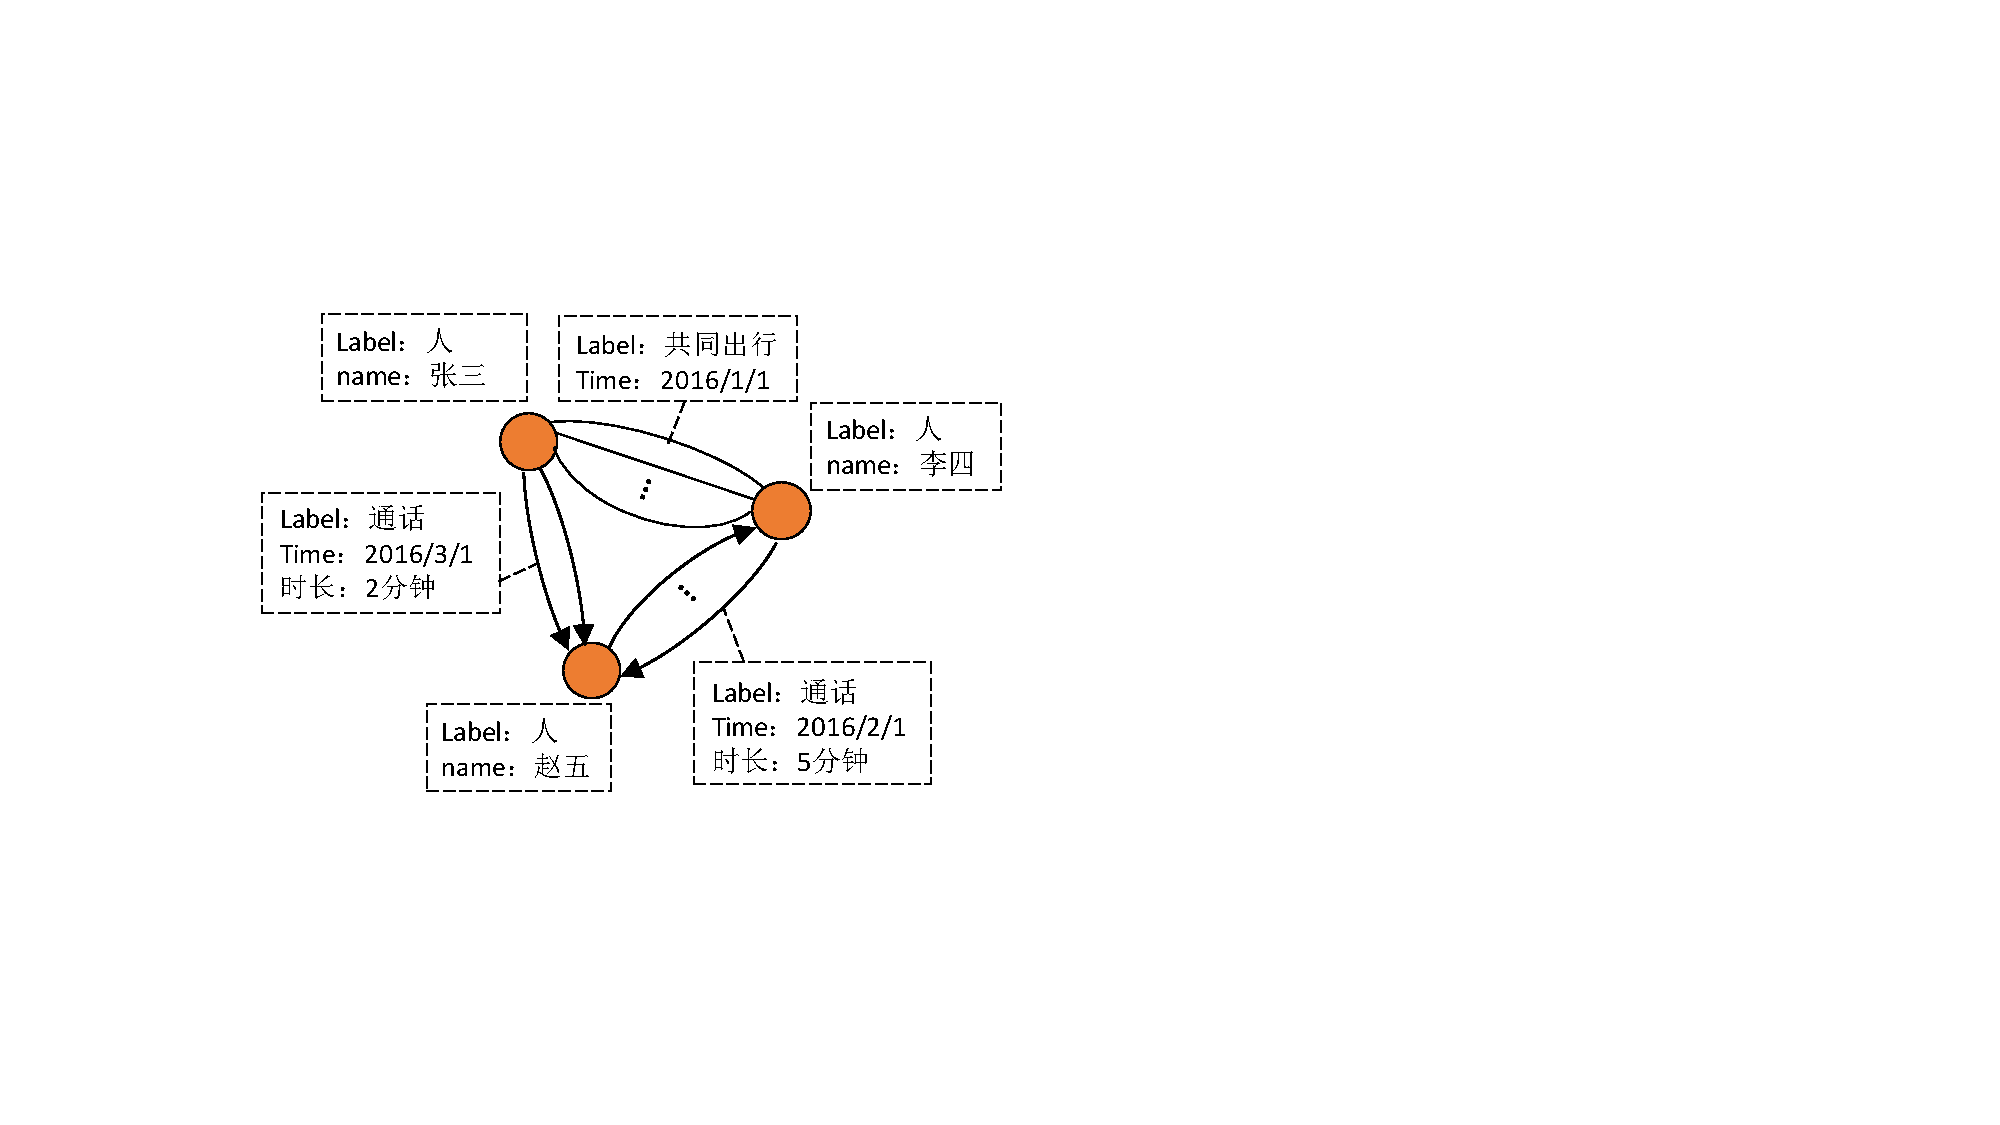
\includegraphics[width=100mm]{fig/property_graph.pdf}
\caption{属性图示例}
\label{fig:property_graph}
\end{figure}

传统解决方案将数据存储在关系型数据库中,如将所有通话数据存储在通话关系表中。关系型数据库能胜任图数据的存储,也能方便地检索元素的内容,但在图结构相关的查询上表现欠佳。比如两跳邻域查询,锁定一个嫌疑人后,要查看其两跳范围内的子图信息。为得到第二跳的邻域结点,需要对各种关系表做昂贵的JOIN操作。图数据库由于其以图的形式存储数据,在图的拓扑结构查询中具有更优异的性能。因此当应用场景中图的拓扑结构查询与元素的内容查询同等重要时,图数据库是最佳的选择。明略数据 是一家大数据解决方案提供商,客户群涵盖刑侦、金融、电信等领域。其中SCOPA 是明略数据的重要产品,在海量刑侦数据上构建起一个数据分析挖掘平台,展现给领域专家的是一张属性图,关联了客户原有的所有数据。SCOPA平台即使用图数据库实现其存储核心。

然而,在富含重边的属性图中,图数据库的查询性能不佳。在传统的图应用中,图中的边一般是稀疏的。如一些公开的图数据集 中,边集的大小约为点集大小的十几倍。但在富含重边的应用场景中,边集大小可能为点集的上万倍。图数据库以邻接表的方式存储图,表中的每一项存储一条边。这使得查询邻接点集时,需要遍历整个邻接表中的所有边。当图中含有大量重边时,邻接表规模巨大,这种数据组织方式导致邻域查询性能严重受损。而邻域查询是大部分图查询的基础,如多跳邻域查询、路径查询、局部聚集系数查询(计算)等,这些查询往往由嵌套的邻域查询实现,随着邻域深度的增加,这种性能受损将被指数级放大。

一种简化重边的建模方式是,将所有同label的重边合并为一条边来表示,边上存储这些重边的所有信息,这样两个实体间的重边数能降低为边的label种类数。然而,将多条重边的数据合并在一条边中存储,会使边的单位数据量骤增,图中的数据粒度过大,同时降低了单条重边的检索和插入效率,每次操作都要先读取相关的所有重边数据,再在其中做查询或插入操作。因此,处理大量重边是一个不可避免的需求。

在许多富含重边的图应用场景中,尽管数据量较大,但数据的操作需求相对单一,而且没有很强的事务性要求。比如在知识图谱的构建中\supercite{knowledge_graph},信息的来源是可靠的,即一旦信息进入知识图谱,则被认为是无需修改的,因此数据操作只需要插入和查询,更新操作很少被执行。在SCOPA的刑侦应用场景中,数据来源是可靠的,且图中数据都是一些客观的事实数据,不需要修改,数据操作主要是图查询和批量的图数据插入。数据插入操作包括原始的全量数据导入和定期的增量数据导入,没有并发的写冲突,也不需要很强的事务性要求。基于上述观察,在放宽了对强事务的支持后,我们可以设计一个相比传统图数据库更为高效的属性图处理系统,来应对含有大量重边的应用场景。

\section{HybriG存储查询架构}
本文提出了一种基于图数据库Titan 和列式存储数据库HBase 的复合存储架构——HybriG。HybriG能从容地处理富含重边的属性图,克服图数据库的局限性,具有更好的查询和插入性能。HyBriG架构应用于SCOPA的底层核心设计,在实践中也验证了其性能的优异性。本文的贡献主要有:分析了图数据库处理大量重边时性能受损的原因,并基于此提出了解决方案HybriG及其存储、查询和高效数据导入设计,最后通过实验验证了HybriG的优异性能。

\section{文章组织结构}
本文组织如下:第2节介绍图数据库相关的预备知识,包括HBase及Titan的实现及其在处理大量重边时的局限性;第3~6节介绍HybriG的系统架构,包括查询模块的设计,数据高效导入方案的设计,以及数据一致性的设计;第7节展示实验结果。第8节介绍大规模图数据处理的相关工作。最后在第9节对本文进行总结。

% vim:ts=4:sw=4
